\documentclass[12pt]{article}
\usepackage[utf8]{inputenc}
\usepackage{amsmath}
\usepackage{amssymb}
\usepackage{multicol}
\usepackage{fullpage}
\usepackage{bera}
\usepackage{xcolor}
\usepackage{hyperref}
\usepackage{tikz}

\setlength{\parindent}{0pt}

\begin{document}

\begin{flushleft}
{\footnotesize Pontificia Universidad Católica de Chile\\
Departamento de Ciencia de la Computación\\
Computación: Ciencia y Tecnología del Mundo Digital\\
}
\begin{center}
{\huge\bf Tarea Chica 3: Máquinas de Turing}\\ \vspace{0.5cm}
Profesor Denis Parra \\
Alumno Diego Bustamante\\

\rule{\linewidth}{0.1mm}
\end{center}
\end{flushleft}

\section*{\small 1.- Explicación del algoritmo de la máquina}

La máquina diseñada posee dos cintas, la primera para recorrer el input y la segunda para almacenar el último número recorrido para poder compararlo con el siguiente. Su objetivo es verificar en una lista de números binarios (de diferente longitud) que, por cada elemento, el que le sigue sea estrictamente mayor.\\

Como se aprecia en el diagrama de estados en la siguiente página, el algoritmo parte en $q_{0}$ como estado inicial. En él, recorrerá la primera cinta y sin importar el dígito, lo copia en la segunda cinta y mientras el original se borra. Si llega a un nuevo número avanza al siguiente estado $punto$ porque hay más números en el input, pero si encuentra el final del input se detiene y termina porque listas de un elemento se deben aceptar.\\

Volviendo al primer caso, una vez copiado el primer elemento, entra en el estado $punto$. En él, el primer cabezal se desplaza por su cinta hasta el final del siguiente elemento sin tomar en cuenta los dígitos.\\

En ese momento pasa al estado $completar$, ambas cintas se devuelven recorriendo ambos números de atrás hacia delante, dejando intacto los dígitos si los encuentra, sino, rellena con ceros para que el largo de ambos sea el mismo.\\

Ahora, al principio de ambos números comienza el estado de $revisar$. Se comparan ambos números, si encuentra que el de la primera cinta es menor que el copiado se rechazará el input, si son iguales seguirá copiando (y borrando el original), sin embargo, si es completamente igual también se rechazará.\\

En un tercer caso, si en $revisar$ se encuentra un 1 en la primera cinta y un 0 en la segunda pasará al estado $mayor$. Este es el único aceptable. El algoritmo continuará copiando y borrando el mayor hasta terminar ambos elementos. Si hay más números en el input (porque encontró un punto) seguirá en el loop del circuito derecho (según el diagrama) pasando al estado $punto$, sino entrará en estado $termina$ y aceptará el input porque el último encontrado es mayor y ya nos habíamos asegurado que los números anteriores cumplían la condición en loops o revisiones ya realizadas.

\vspace{4ex}

\begin{center}
	\textbf{Diagrama de estados}
	\vspace{3ex}
	
	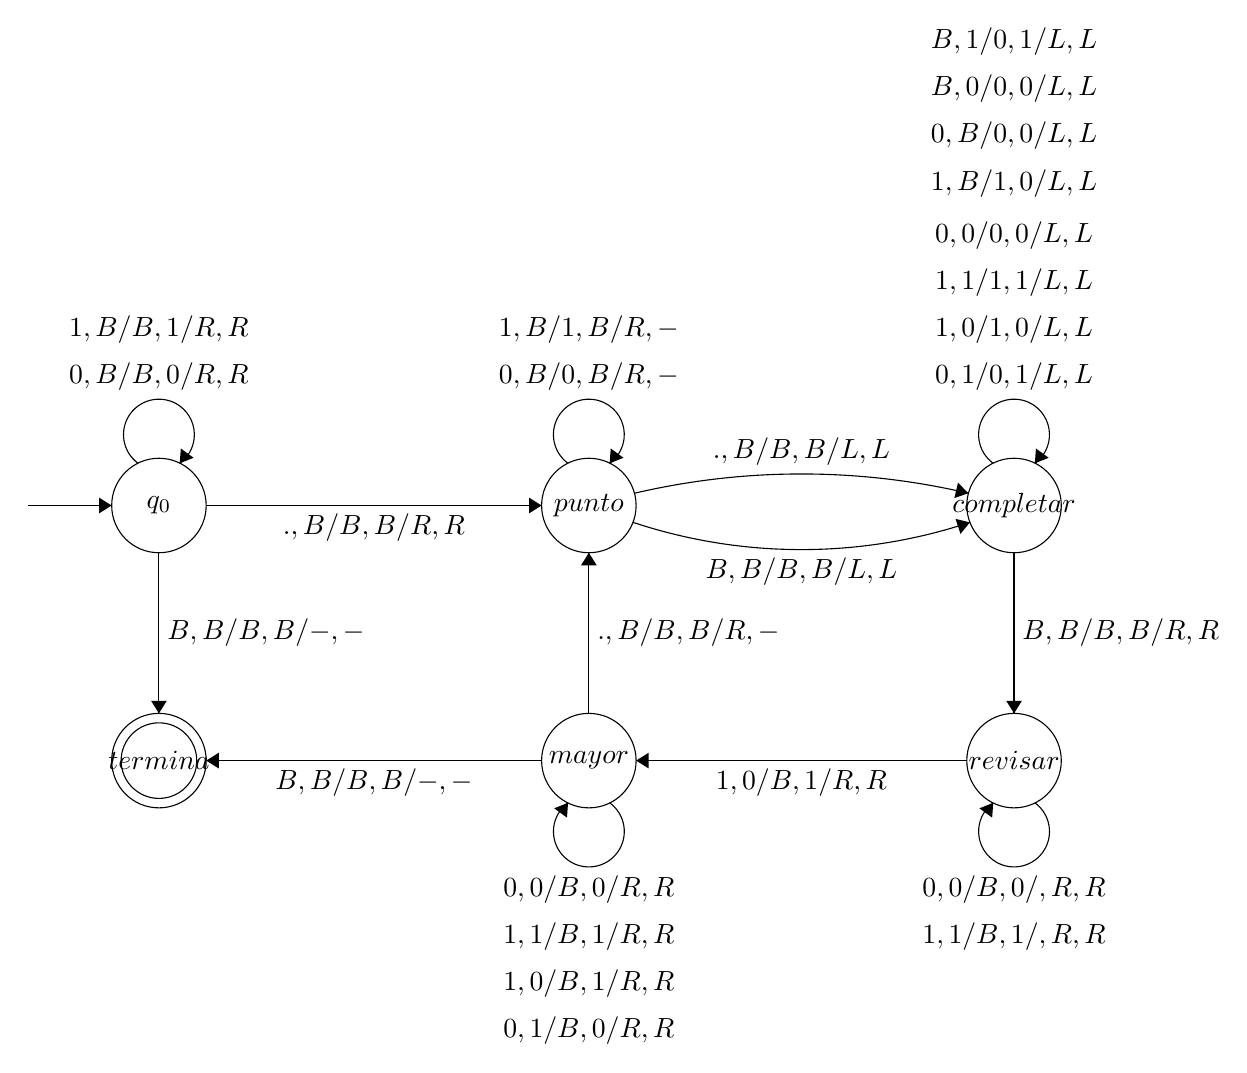
\begin{tikzpicture}[scale=0.2]
	\tikzstyle{every node}+=[inner sep=0pt]
	\draw [black] (11.1,-18.4) circle (3);
	\draw (11.1,-18.4) node {$q_0$};
	\draw [black] (38.4,-18.4) circle (3);
	\draw (38.4,-18.4) node {$punto$};
	\draw [black] (65.4,-18.4) circle (3);
	\draw (65.4,-18.4) node {$completar$};
	\draw [black] (65.4,-34.6) circle (3);
	\draw (65.4,-34.6) node {$revisar$};
	\draw [black] (38.4,-34.6) circle (3);
	\draw (38.4,-34.6) node {$mayor$};
	\draw [black] (11.1,-34.6) circle (3);
	\draw (11.1,-34.6) node {$termina$};
	\draw [black] (11.1,-34.6) circle (2.4);
	\draw [black] (2.8,-18.4) -- (8.1,-18.4);
	\fill [black] (8.1,-18.4) -- (7.3,-17.9) -- (7.3,-18.9);
	\draw [black] (14.1,-18.4) -- (35.4,-18.4);
	\fill [black] (35.4,-18.4) -- (34.6,-17.9) -- (34.6,-18.9);
	\draw (24.75,-18.9) node [below] {$.,B/B,B/R,R$};
	\draw [black] (9.777,-15.72) arc (234:-54:2.25);
	\draw (11.1,-8.15) node [above] {$1,B/B,1/R,R$};
	\draw (11.1,-11.15) node [above] {$0,B/B,0/R,R$};
	\fill [black] (12.42,-15.72) -- (13.3,-15.37) -- (12.49,-14.78);
	\draw [black] (62.599,-19.47) arc (-71.62029:-108.37971:33.93);
	\fill [black] (62.6,-19.47) -- (61.68,-19.25) -- (62,-20.2);
	\draw (51.9,-21.7) node [below] {$B,B/B,B/L,L$};
	\draw [black] (65.4,-21.4) -- (65.4,-31.6);
	\fill [black] (65.4,-31.6) -- (65.9,-30.8) -- (64.9,-30.8);
	\draw (65.9,-26.5) node [right] {$B,B/B,B/R,R$};
	\draw [black] (62.4,-34.6) -- (41.4,-34.6);
	\fill [black] (41.4,-34.6) -- (42.2,-35.1) -- (42.2,-34.1);
	\draw (51.9,-35.1) node [below] {$1,0/B,1/R,R$};
	\draw [black] (35.4,-34.6) -- (14.1,-34.6);
	\fill [black] (14.1,-34.6) -- (14.9,-35.1) -- (14.9,-34.1);
	\draw (24.75,-35.1) node [below] {$B,B/B,B/-,-$};
	\draw [black] (38.4,-31.6) -- (38.4,-21.4);
	\fill [black] (38.4,-21.4) -- (37.9,-22.2) -- (38.9,-22.2);
	\draw (38.9,-26.5) node [right] {$.,B/B,B/R,-$};
	\draw [black] (37.077,-15.72) arc (234:-54:2.25);
	\draw (38.4,-8.15) node [above] {$1,B/1,B/R,-$};
	\draw (38.4,-11.15) node [above] {$0,B/0,B/R,-$};
	\fill [black] (39.72,-15.72) -- (40.6,-15.37) -- (39.79,-14.78);
	\draw [black] (64.077,-15.72) arc (234:-54:2.25);
	\draw (65.4,10.15) node [above] {$B,1/0,1/L,L$};
	\draw (65.4,7.15) node [above] {$B,0/0,0/L,L$};
	\draw (65.4,4.15) node [above] {$0,B/0,0/L,L$};
	\draw (65.4,1.15) node [above] {$1,B/1,0/L,L$};
	\draw (65.4,-2.15) node [above] {$0,0/0,0/L,L$};
	\draw (65.4,-5.15) node [above] {$1,1/1,1/L,L$};
	\draw (65.4,-8.15) node [above] {$1,0/1,0/L,L$};
	\draw (65.4,-11.15) node [above] {$0,1/0,1/L,L$};
	\fill [black] (66.72,-15.72) -- (67.6,-15.37) -- (66.79,-14.78);
	\draw [black] (11.1,-21.4) -- (11.1,-31.6);
	\fill [black] (11.1,-31.6) -- (11.6,-30.8) -- (10.6,-30.8);
	\draw (11.6,-26.5) node [right] {$B,B/B,B/-,-$};
	\draw [black] (41.297,-17.622) arc (103.18773:76.81227:46.476);
	\fill [black] (62.5,-17.62) -- (61.84,-16.95) -- (61.61,-17.93);
	\draw (51.9,-15.9) node [above] {$.,B/B,B/L,L$};
	\draw [black] (66.723,-37.28) arc (54:-234:2.25);
	\draw (65.4,-41.85) node [below] {$0,0/B,0/,R,R$};
	\draw (65.4,-44.85) node [below] {$1,1/B,1/,R,R$};
	\fill [black] (64.08,-37.28) -- (63.2,-37.63) -- (64.01,-38.22);
	\draw [black] (39.723,-37.28) arc (54:-234:2.25);
	\draw (38.4,-41.85) node [below] {$0,0/B,0/R,R$};
	\draw (38.4,-44.85) node [below] {$1,1/B,1/R,R$};
	\draw (38.4,-47.85) node [below] {$1,0/B,1/R,R$};
	\draw (38.4,-50.85) node [below] {$0,1/B,0/R,R$};
	\fill [black] (37.08,-37.28) -- (36.2,-37.63) -- (37.01,-38.22);
	\end{tikzpicture}
\end{center}

\pagebreak


\section*{\small 2.- Definición formal de la máquina}


$M=(Q,\Gamma,\Sigma,q_{0},\delta,F)$\\
 
Con:\\

$Q=\{q_{0}, punto, completar, revisar, mayor, termina\}$ \\
$\Gamma=\{0,1,.,B\}$ \\
$q_{0}=q_{0}$ \\
$F=\{termina\}$ \\

\vspace{2ex}


\section*{\small 3.- Descripción de los estados}

 Primero, parte en un estado inicial $q_{0}$. Como se aprecia en la tabla en las siguien-tes páginas en este estado la máquina recorre el primer número del input hacia la derecha. Mientras encuentre un 0 o un 1 y lo almacena escribiendo el dígito encontrado en la segunda cinta de izquierda a derecha (ambas direcciones son $\rightarrow$, $\rightarrow$). En $q_{0}$ se encontrará sólo B en la segunda cinta por eso todos los símbolos actuales son del tipo (X,B). Además, los dígitos del primer número se reemplazan por B para que no se solapen en las siguientes etapas. Si encuentra (B,B) en $q_{0}$, entonces, se pasará al estado $termina$ (estado final, caracterizado al final de la tabla), se mantiene ahí (-,-) y retorna Aceptado, ya que una lista de un elemento cumple la condición.\\ 

Segundo, si en $q_{0}$ encuentra "." en la primera cinta (que es inmediatamente intercambiado por B) entrará en estado $punto$, además de realizar un movimiento $\rightarrow$, -. En él, avanzará hasta el siguiente "." o B en la primera cinta para poder comparar el largo del siguiente número con el copiado. En $punto$ no interesan los dígitos, el primer cabezal se traslada por ellos mientras que el segundo no se mueve.\\

Tercero, al encontrar el siguiente "." o B en la primera cinta entra en estado $completar$. En él, se reescriben ambos números en dirección $\leftarrow$,$\leftarrow$ cualesquiera sean las combinaciones de ceros y unos (ver $completar$ en la tabla). Pero, si encuentra espacios vacíos en uno sólo de los números, esto es, (B,X) o (X,B) rellena ese vacío con ceros hasta que ambos largos sean iguales, es decir, al encontrar (B,B). Al terminar se cambiará al siguiente estado.\\

Cuarto, entra en estado $revisar$ en dirección $\rightarrow$,$\rightarrow$. En él, los 2 cabezales avanzarán hasta el final de ambos números y mientras se les compara. El primero lo copiará en el segundo, además de siempre escribir B en la primera cinta como en $punto$. Si la lista termina en este estado entonces no se define un final como se aprecia en la tabla pues esto significa que los números eran iguales y debe rechazar el input. Si se encuentra (0,1) también retorna Rechazado puesto que no está definido porque el copiado sería mayor. Por otro lado, si encuentra un 1 en el input y 0 en la copia significa que es mayor y se pasará al siguiente estado.\\

Quinto, ya establecido que el siguiente numero es $mayor$, se entra en ese estado. Sólo resta seguir copiando el número como en $revision$ en dirección $\rightarrow$,$\rightarrow$ y llegar al final de ambos elementos, esto es, (.,B) o (B,B). Si encuentra (B,B) retornará Aceptado, ya que, pasó la revisión siendo mayor y accede al estado $termina$ en movimiento -,-. Finalmente, si se encuentra con (.,B) entrará en estado $punto$ y se repetirá todo desde el segundo paso.\\

El estado $termina$ es en el que se acepta el input. Cómo se accede a él es descrito en el estado $q_{0}$ y $mayor$.

\vspace{5ex}

La función $\delta$ se define según la siguiente tabla:\\

\begin{center}
	\begin{tabular}{ |c|c|c|c|c| }
		\hline
		\multicolumn{5}{|c|}{\textbf{Tabla 1: Función $\delta$ (transiciones)}}\\
		\hline
		Estado actual & S actual & S nuevo & Estado siguiente & Dirección\\
		\hline
		$q_{0}$ & 0,B & B,0 & $q_{0}$ & $\rightarrow$,$\rightarrow$\\
		$q_{0}$ & 1,B & B,1 & $q_{0}$ & $\rightarrow$,$\rightarrow$\\
		$q_{0}$ & .,B & B,B & $punto$ & $\rightarrow$,-\\
		\hline
		$punto$ & 0,B & 0,B & $punto$ & $\rightarrow$,-\\
		$punto$ & 1,B & 1,B & $punto$ & $\rightarrow$,-\\
		$punto$ & .,B & .,B & $completar$ & $\leftarrow$,$\leftarrow$\\
		$punto$ & B,B & B,B & $completar$ & $\leftarrow$,$\leftarrow$\\
		\hline
		$comlpetar$ & 0,1 & 0,1 & $completar$ & $\leftarrow$,$\leftarrow$\\
		$comlpetar$ & 1,0 & 1,0 & $completar$ & $\leftarrow$,$\leftarrow$\\
		$comlpetar$ & 1,1 & 1,1 & $completar$ & $\leftarrow$,$\leftarrow$\\
		$comlpetar$ & 0,0 & 0,0 & $completar$ & $\leftarrow$,$\leftarrow$\\
		$comlpetar$ & 1,B & 1,0 & $completar$ & $\leftarrow$,$\leftarrow$\\
		$comlpetar$ & 0,B & 0,0 & $completar$ & $\leftarrow$,$\leftarrow$\\
		$comlpetar$ & B,1 & 0,1 & $completar$ & $\leftarrow$,$\leftarrow$\\
		$comlpetar$ & B,0 & 0,0 & $completar$ & $\leftarrow$,$\leftarrow$\\
		$comlpetar$ & B,B & B,B & $revisar$ & $\rightarrow$,$\rightarrow$\\
		\hline
		$revisar$ & 0,0 & B,0 & $revisar$ & $\rightarrow$,$\rightarrow$\\
		$revisar$ & 1,1 & B,1 & $revisar$ & $\rightarrow$,$\rightarrow$\\
		$revisar$ & 1,0 & B,1 & $mayor$ & $\rightarrow$,$\rightarrow$\\
		\hline
	\end{tabular} 
\end{center}

\begin{center}
	\begin{tabular}{ |c|c|c|c|c| }
		\hline
		Estado actual & S actual & S nuevo & Estado siguiente & Dirección\\
		\hline
		$mayor$ & 0,0 & B,0 & $mayor$ & $\rightarrow$,$\rightarrow$\\
		$mayor$ & 1,1 & B,1 & $mayor$ & $\rightarrow$,$\rightarrow$\\
		$mayor$ & 1,0 & B,1 & $mayor$ & $\rightarrow$,$\rightarrow$\\
		$mayor$ & 0,1 & B,0 & $mayor$ & $\rightarrow$,$\rightarrow$\\
		$mayor$ & .,B & B,B & $punto$ & $\rightarrow$,-\\
		\hline
		$mayor$ & B,B & B,B & $termina$ & -,-\\
		$q_{0}$ & B,B & B,B & $termina$ & -,-\\
		\hline
	\end{tabular} 
\end{center}

\end{document}
